\section{Modellbildung Würfelseite}
Die Untersuchung des Systems beginnt mit der Bestimmung eines mathematischen Modells, welches in diesem Abschnitt näher erläutert wird. Die Herleitung der Systemdynamik erfolgt mit Hilfe der Methoden nach Kane. Zunächst beschränkt sich die mechanische Untersuchung auf einen vereinfachten Prototypen, welcher aus einer Würfelseite besteht, die auf einer Achse gelagert ist. An der Würfelseite ist ein Motor befestigt, auf wessen Schaft wiederum eine Schwungmasse gelagert ist.

\begin{figure}[!h]
\centering
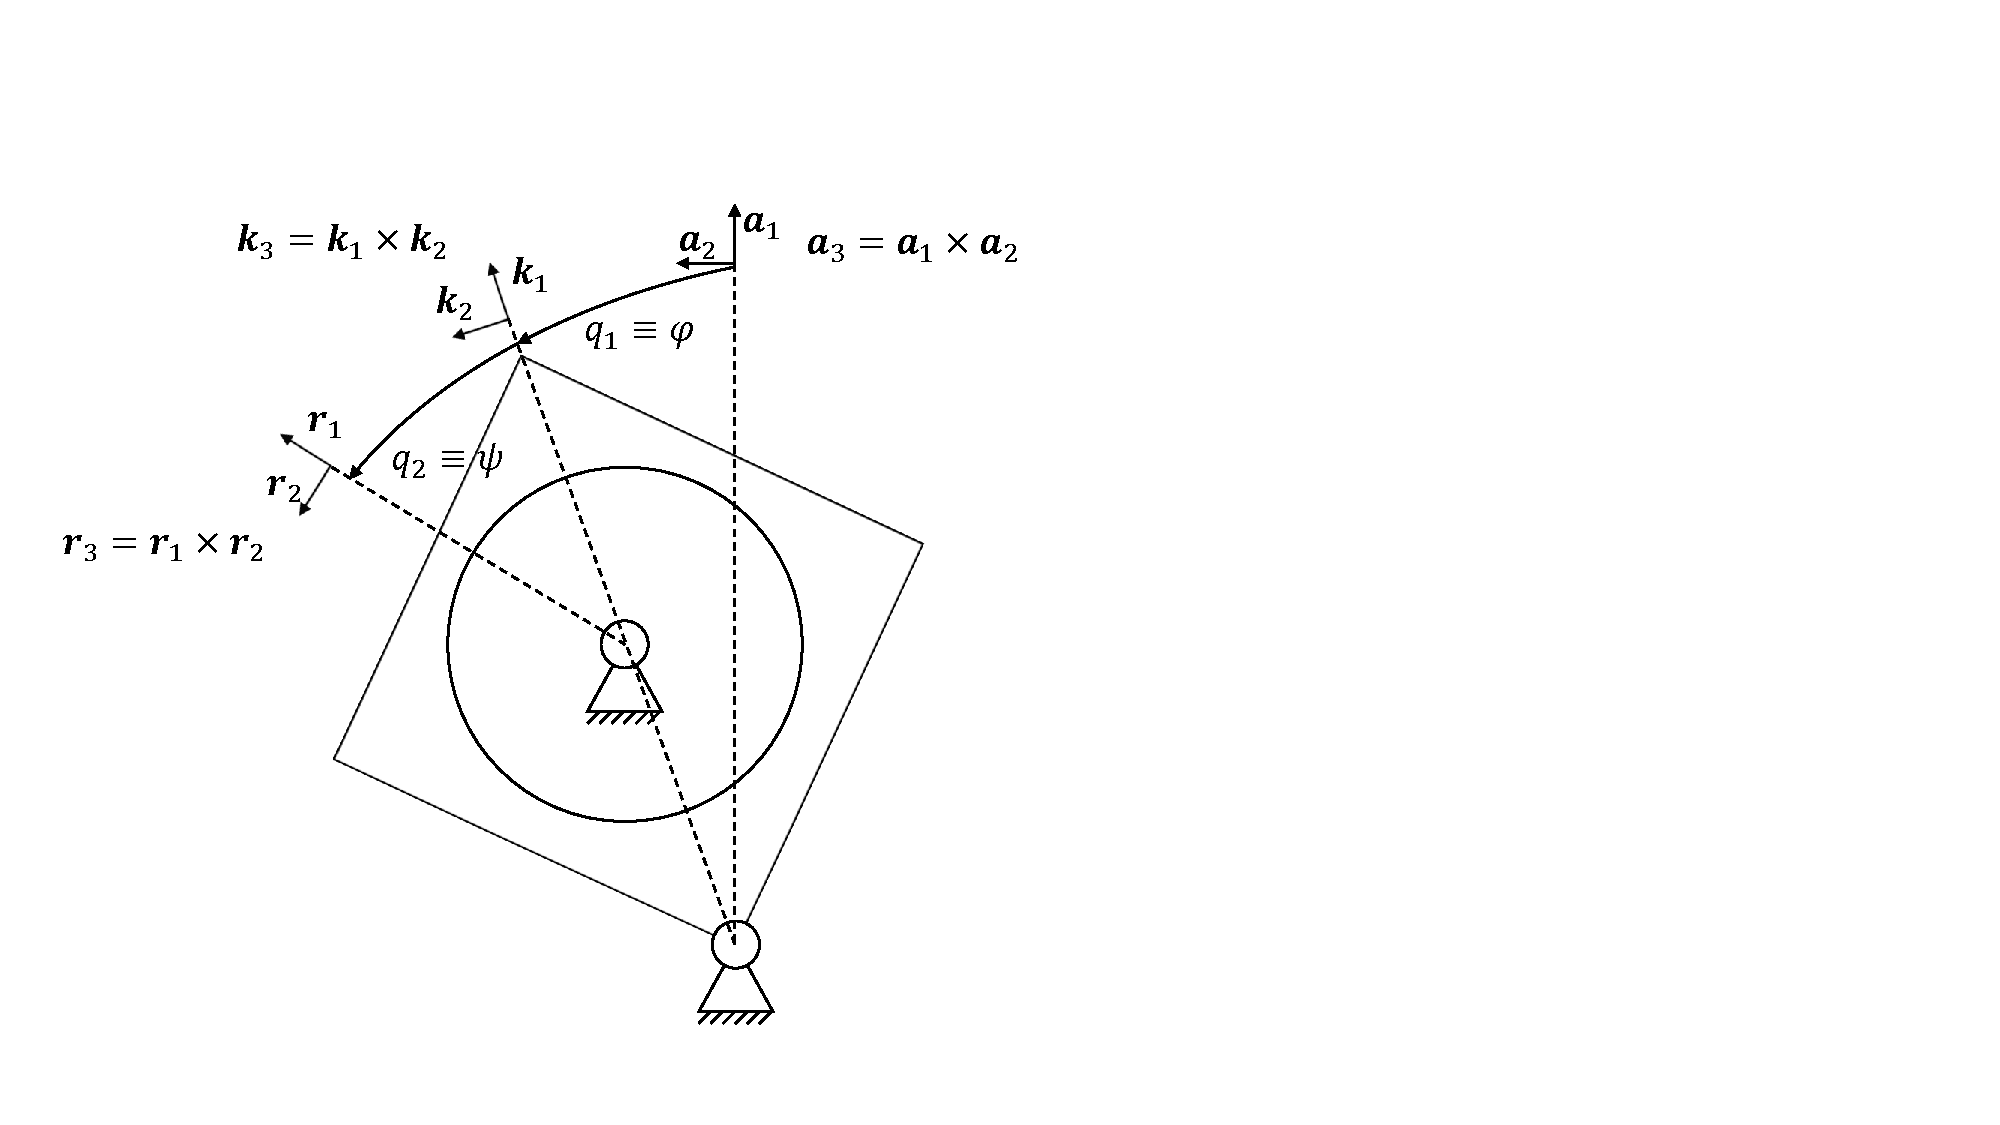
\includegraphics[width=0.6\linewidth, trim={1cm 1.5cm 18cm 3.5cm}, clip]{2_ModellWuerfelseite/img/ModellWuerfelseite}
\caption{Mechanischer Aufbau der Würfelseite, Quelle: eigene Darstellung}
\end{figure}

Zu Beginn werden der Untersuchung werden die Bezugssysteme festgelegt, welche durch drei, paarweise orthogonale, Einheitsvektoren definiert sind. Die Vektorbasis eines Bezugssystem dient als eine Art Einheit um vektorielle Größen, wie z.B. Position oder Geschwindigkeit, darzustellen. Das untersuchte System verfügt über das raumfeste Bezugssystem $A$, welches durch die drei Einheitsvektoren $\bs{a}_1$, $\bs{a}_2$ und $\bs{a}_3$ definiert wird. An der Würfelseite ist ein weiteres Bezugssystem $K$ fixiert, dessen Vektorbasis aus $\bs{k}_1$, $\bs{k}_2$ und $\bs{k}_3$ besteht. Zuletzt ist das, aus den Einheitsvektoren $\bs{r}_1$, $\bs{r}_2$ und $\bs{r}_3$ bestehende, Bezugssystem $R$ zu nennen, welches auf der Schwungmasse fixiert ist. 

Das holonome System verfügt über zwei rotatorische Freiheitsgrade, welche mit Hilfe der generalisierten Koordinaten $q_1 = \varphi$ und $q_2 = \psi$ beschrieben werden. Der Winkel $\varphi$ beschreibt die Rotation der Würfelseite um den Punkt $O$. Die Rotation der Schwungmasse $R$ relativ zu der Würfelseite wird von dem Winkel $\psi$ beschrieben. Mit Hilfe der generalisierten Koordinaten ist es möglich einen Vektor, welcher in einem Bezugssystem dargestellt ist, in ein zweites Bezugssystem zu projizieren. Als Beispiel soll die Position des Schwerpunktes von $K$ dienen, welche von dem Vektor $\bs{c}_K$ beschrieben wird. Mit Hilfe des Skalarproduktes eines Vektors mit einem Einheitsvektors, kann der Betrag des Vektors in Richtung des Einheitvektors ermittelt werden. Folglich können somit die Komponenten eines Vektors in einem beliebigen Bezugssystem dargestellt werden.

\begin{equation}
\bs{c}_K = \vecBS{K}{l_{AC}}{0}{0} = \vecBS{A}{\bs{c}_K \cdot \bs{a}_1}{\bs{c}_K \cdot \bs{a}_2} {\bs{c}_K \cdot \bs{a}_3} = \begin{pmatrix}
\bs{a}_1 \cdot \bs{k}_1 & \bs{a}_1 \cdot \bs{k}_2 & \bs{a}_1 \cdot \bs{k}_3 \\
\bs{a}_2 \cdot \bs{k}_1 & \bs{a}_2 \cdot \bs{k}_2 & \bs{a}_2 \cdot \bs{k}_3 \\
\bs{a}_3 \cdot \bs{k}_1 & \bs{a}_3 \cdot \bs{k}_2 & \bs{a}_3 \cdot \bs{k}_3 \\
\end{pmatrix} \cdot \bs{c}_K = \pMat{K}{A} \cdot \bs{c}_K
\end{equation}

Die Projektion kann somit in Form einer Matrix $\pMat{K}{A}$ dargestellt werden, welche aus den Skalarprodukten der Einheitsvektoren besteht. Die umgekehrte Projektion kann mit Hilfe der Matrix $\pMat{A}{K}$ durchgeführt werden, welche die Transponierte von $\pMat{A}{K}$ ist. Die Projektionsmatrizen des ursprünglichen Systems sind die folgenden.

\begin{equation}
\pMat{A}{K} = \begin{pmatrix}
c_{\varphi} && s_{\varphi} && 0 \\ -s_{\varphi} && c_{\varphi} && 0 \\ 0 && 0 && 1
\end{pmatrix} \hspace{15pt}
\pMat{K}{R} = \begin{pmatrix}
c_{\psi} && s_{\psi} && 0 \\ -s_{\psi} && c_{\psi} && 0 \\ 0 && 0 && 1
\end{pmatrix}
\end{equation}

Somit kann nun auch der Schwerpunkt der Würfelseite in dem raumfesten Bezugssystem $A$ dargestellt werden.

\begin{equation}
\bs{C}_K = \vecBS{K}{l_{AC}}{0}{0} = \presuper{A}{\begin{pmatrix}
\pMat{K}{A} \cdot \vecBS{K}{l_{AC}}{0}{0}
\end{pmatrix}} = \vecBS{A}{c_{\varphi} \cdot l_{AC}}{s_{\varphi} \cdot  l_{AC}}{0}
\end{equation}

An diesem Beispiel ist bereits zu erkennen, von welcher Bedeutung Bezugssysteme bei der Darstellung von Vektoren sind. Die Position des Schwerpunktes ist aus Sicht der Würfelseite konstant, jedoch ist seine Position im raumfesten Bezugssystem $A$ von dem Winkel $\varphi$ abhängig. Im Kehrschluss ist die Darstellung eines Vektors nur unter Angabe eines Bezugssystem sinnvoll.

Nachdem die Position bzw. Orientierung der Körper mit Hilfe der generalisierten Koordinaten bestimmt wurde besteht der nächste Schritt darin, die Geschwindigkeiten der beiden Körper zu bestimmen. Die Geschwindigkeit eines Körpers ist abhängig von dem Bezugssystem in welchem er sich bewegt. Folglich muss das Bezugssystem in wessen Relation sich ein Körper bewegt, bei der Darstellung der Geschwindigkeit berücksichtigt werden. Als Beispiel dient die Geschwindigkeit der Schwungmasse relativ zu der Würfelseite $\vel{K}{\bs{\omega}}{R}$, die Geschwindigkeit der Schwungmasse im raumfesten Bezugssystem $\vel{A}{\bs{\omega}}{R}$ und die Geschwindigkeit der Würfelseite in $A$, $\vel{A}{\bs{\omega}}{K}$.

\begin{equation}
\vel{K}{\bs{\omega}}{R} = \vecBS{A}{0}{0}{\dot{\psi}} \hspace{15pt} \vel{A}{\bs{\omega}}{K} = \vecBS{A}{0}{0}{\dot{\varphi}} \hspace{15pt} \vel{A}{\bs{\omega}}{R} = \vel{K}{\bs{\omega}}{R} + \vel{A}{\bs{\omega}}{K} = \vecBS{A}{0}{0}{\dot{\varphi}+\dot{\psi}}
\end{equation}

Es sei vermerkt, dass eine Geschwindigkeit in einem beliebigen Bezugssystem dargestellt werden kann, es handelt sich allerdings nach wie vor um die Geschwindigkeit des Körpers in dem ursprünglichen Bezugssystem, lediglich die Darstellung wurde verändert.

Um die Darstellung der Geschwindigkeiten zu vereinfachen, werden die generalisierten Geschwindigkeiten $u_1 \equiv \dot{\varphi}$ und $u_2 \equiv \dot{\psi}$ definiert. Somit ist es möglich die Geschwindigkeiten der Schwungmasse $\vel{A}{\bs{\omega}}{R}$ und der Würfelseite $\vel{A}{\bs{\omega}}{K}$ als Summe der generalisierten Geschwindigkeiten $u_i$ und der partiellen Geschwindigkeiten $\vel{A}{\bs{\omega}}{R}_i$ und $\vel{A}{\bs{\omega}}{K}_i$.

\begin{equation}
\vel{A}{\bs{\omega}}{K} = \dot{\varphi} \cdot \bs{a}_3 + \dot{\psi} \cdot 0 \hspace{5pt} \rightarrow \hspace{5pt} \vel{A}{\bs{\omega}}{K}_1 = \bs{a}_3 \hspace{15pt} \vel{A}{\bs{\omega}}{K}_2 = 0
\end{equation} 
\begin{equation}
\vel{A}{\bs{\omega}}{R} = \dot{\varphi} \cdot \bs{a}_3 + \dot{\psi} \cdot \bs{a}_3 \hspace{5pt} \rightarrow \hspace{5pt} \vel{A}{\bs{\omega}}{R}_1 = \bs{a}_3 \hspace{15pt}  \vel{A}{\bs{\omega}}{R}_2 = \bs{a}_3
\end{equation}

Bei den generalisierten Geschwindigkeiten $\dot{\varphi}$ und $\dot{\psi}$ handelt es sich um Skalare. Sie beschreiben die komponentenweise Zusammensetzung der Geschwindigkeiten der beiden Körper. Die partiellen Geschwindigkeiten hingegen sind Vektoren, welche die Orientierung der generalisierten Geschwindigkeiten wiedergeben und somit deren Beitrag zu der Bewegung in Richtung der Freiheitsgrade darstellen.

Der nächste Schritt besteht darin, die Drehmomente zu untersuchen, welche auf die Würfelseite und die Schwungmasse wirken. Mit Hilfe der wirkenden Kräfte können letzten Endes die Bewegungsgleichungen ermittelt werden.

Die Bewegung der Schwungmasse wird einerseits durch das Motormoment $\bs{T}^{R/M}_M$ beeinflusst, andererseits wird sie von der Reibung in $M$ durch das Drehmoment $\bs{T}^{R/M}_R$ verzögert. Das Reibmoment wird als proportional zur Geschwindigkeit $\dot{\psi}$ modelliert. Somit ergibt sich das resultierende Drehmoment $\bs{T}_R$.

\begin{equation}
\bs{T}^{R/M} = \bs{T}^{R/M}_M + \bs{T}^{R/M}_R = (T_M + C_{\psi} \cdot \dot{\psi})\cdot \bs{a}_3
\end{equation}

Das Motormoment $\bs{T}_M$ und das Reibmoment $\bs{R}_R$ wirken in umgekehrter Richtung auf die Würfelseite. Zusätzlich wird diese von dem Gravitationsmoment $\bs{T}^{K/O}_G$ und dem Reibmoment der Würfelseite $\bs{T}^{K/O}_R$. Aus der Summe dieser Komponenten ergibt sich das resultierende Drehmoment $\bs{T}^{K/O}$.

\begin{equation}
\bs{T}^{K/O} = \bs{T}^{K/O}_G - \bs{T}^{K/O}_R - \bs{T}^{R/M}_M + \bs{T}^{R/M}_R = 
(m_G \cdot g \cdot l_{AC} \cdot s_{\varphi} - C_{\varphi} \cdot \dot{\varphi} - T_M + C_{\psi} \cdot \dot{\psi}) \cdot \bs{a}_3
\end{equation}

Über das Skalarprodukt der resultierenden Drehmomente und der partiellen Geschwindigkeiten können die generalisierten aktiven Kräfte $F_1$ und $F_2$ berechnet werden. Diese stellen den Einfluss der wirkenden Kräfte und Momente auf die generalisierten Geschwindigkeiten $\dot{\varphi}$ und $\dot{\psi}$ dar.

\begin{equation}
F_1 = \vel{A}{\bs{\omega}}{K}_1 \cdot \bs{T}^{K/O} + \vel{A}{\bs{\omega}}{R}_1 \cdot \bs{T}^{R/M}= m_G \cdot g \cdot l_{AC} \cdot s_{\varphi} - C_{\varphi} \cdot \dot{\varphi}
\end{equation}
\begin{equation}
F_2 = \vel{A}{\bs{\omega}}{K}_2 \cdot \bs{T}^{K/O} + \vel{A}{\bs{\omega}}{R}_2 \cdot \bs{T}^{R/M}= T_M - C_{\psi} \cdot {\dot{\psi}}
\end{equation}

Die letztendlichen Bewegungsgleichungen werden über das Gleichgewicht der generalisierten, aktiven Kräfte und der generalisierten Trägheitskräfte gewonnen. Folglich muss zuletzt das Trägheitsmoment der Schwungmasse $\bs{T}^*_R$ und der Würfelseite $\bs{T}^*_K$ bestimmt werden. Ersteres ergibt sich aus dem Massenträgheitsmoment $I^{R/M}$ der Schwungmasse um den Punkt $M$ und seiner Winkelbeschleunigung in $A$.

\begin{equation}
\bs{T}^*_R = -I^{R/M} \cdot \vecBS{A}{0}{0}{\ddot{\varphi} + \ddot{\psi}}
\end{equation}

Das Trägheitsmoment der Würfelseite hängt von ihrer Winkelbeschleunigung in $A$,ihrem Massenträgheitsmoment $I^{K/O}$ um $O$ und der Position bzw. dem Gewicht der Schwungmasse ab.

\begin{equation}
\bs{T}^*_K = -(I^{K/O} + m_R \cdot l_{AB}^2) \cdot \vecBS{A}{0}{0}{\ddot{\varphi}}
\end{equation}

Die generalisierten Trägheitskräfte $F^*_1$ und $F^*_2$ ergeben sich wiederum durch die Skalarmuliplikation mit den partiellen Geschwindigkeiten. Das heißt die Trägheitsmomente der beiden Körper werden in die Bewegungsrichtung der generalisierten Geschwindigkeiten, also der Freiheitsgrade, projiziert.

\begin{equation}
F^*_1 = \vel{A}{\omega}{K}_1 \cdot \bs{T}^*_K + \vel{A}{\omega}{R}_1 \cdot \bs{T}^*_R = -(I^{K/O} + I^{R/M} + m_R \cdot l_{AB}^2)\cdot \ddot{\varphi} - I^{R/M} \cdot \ddot{\psi}
\end{equation}
\begin{equation}
F^*_2 = \vel{A}{\omega}{K}_2 \cdot \bs{T}^*_K + \vel{A}{\omega}{R}_2 \cdot \bs{T}^*_R = -I^{R/M}\cdot(\ddot{\varphi}+\ddot{\psi})
\end{equation}

Die Bewegungsgleichungen ergeben sich nun aus der Summe der generalisierten aktiven Kräften $F_i$ und der generalisierten Trägheitskräfte $F^*_i$. Die Aussage dieser Gleichungen besteht darin, dass die Projektion, der wirkenden Kräfte in Richtung der partiellen Geschwindigkeiten, gleich der Projektion der Impulsänderung in Richtung der partiellen Geschwindigkeiten ist.

\begin{equation}
F_1 + F^*_1 = 0 \hspace{5pt} \rightarrow \hspace{5pt} (I^{K/O}+I^{R/M}+m_R\cdot l_{AB}^2)\cdot \ddot{\varphi} = m_G \cdot g \cdot l_{AC} \cdot s_{\varphi} - C_{\varphi} \cdot \dot{\varphi} - I^{R/M} \cdot \ddot{\psi}
\end{equation}
\begin{equation}
F_2 + F^*_2 = 0 \hspace{5pt} \rightarrow \hspace{5pt} I^{R/M} \cdot \ddot{\psi} = T_M - C_{\psi} \cdot \dot{\psi} - I^{R/M} \cdot \ddot{\varphi}
\end{equation}